%%%%%%%%%%%%%%%%%%%%%%%%%%%%%%%%%%%%%%%%%%%%%%%%%%%%%%%%%%%%%%%%%%%%%%%%%%%%%%%%
% Chapter 3: Recursos y herramientas
%%%%%%%%%%%%%%%%%%%%%%%%%%%%%%%%%%%%%%%%%%%%%%%%%%%%%%%%%%%%%%%%%%%%%%%%%%%%%%%%

%+++++++++++++++++++++++++++++++++++++++++++++++++++++++++++++++++++++++++++++++
% \section{ROS}
% \label{3:sec:3}
ROS (Robot Operating System) es un framework de código abierto diseñado para
realizar software robótico. Entre las principales funcionalidades destacan una
abstracción del hardware, el control de dispositivos, paso de mensajes entre los
procesos y una gran variedad de herramientas y librerías. Por otra parte ROS
cuenta con un sistema de paquetes, que permite instalar, compilar e incluso
modificar paquetes externos creados por la comunidad \cite{ROSAbout}.

El objetivo principal es permitir la abstracción y la simplificación de  muchas
de las tareas que conllevan construir un robot de forma independiente, uno de
los principales problemas que llevan a condenar al fracaso este tipo de
proyectos, mediante el desarrollo de software colaborativo. En definitiva, ROS
promueve la reutilización de código para evitar tener que reinventar la rueda a
los desarrolladores y científicos en cada nuevo proyecto \cite{ROSIntro}.

De esta forma, a modo de ejemplo un grupo de desarrolladores puede trabajar e
investigar en la construcción de mapas, mientras que en otra parte del mundo,
otro grupo de expertos puede estar especializado en la localización con el uso
de mapas. Ambos comparten el conocimiento entre ambos y con el resto de la
comunidad para conseguir mejores resultados en conjunto.

El software de ROS se distribuye de la siguiente manera:

\begin{itemize}
  \item Herramientas y lenguajes independientes para construir y distribuir ROS.
  \item Librerías del cliente de ROS que facilitan el desarrollo.
  \item Paquetes que contienen la aplicación del usuario.
\end{itemize}

Tanto las herramientas como las librerías del cliente de ROS están escritas
principalmente en C++ y Python. Las librerías principales de ROS siguen los
principios Unix-like ya que la mayoría de dependencias son proyectos de código
abierto, permitiendo que muchas distribuciones distribuyan las librerías y
paquetes de ROS \cite{ROSWiki}.

ROS ha sido diseñado para ser un sistema distribuido lo más modular posible,
permitiendo que los usuarios puedan utilizar lo justo y necesario, desde los
paquetes del núcleo y la comunidad, hasta utilizar sus propios paquetes
personales. Actualmente ROS cuenta con más de 3000 paquetes públicos en su
ecosistema, siendo difícil conocer cual es el número real de todos los paquetes.
Muchos de estos paquetes ayudan enormemente en la infraestructura de la
comunidad, ofreciendo accesos a drivers de dispositivo, capacidades genéricas en
robótica, algoritmos, herramientas de desarrollo y librerías.

Desde sus inicios, la comunidad de ROS ha crecido considerablemente en todo el
mundo, principalmente en laboratorios de investigación, pero en los últimos
tiempos también en otros sectores comerciales e industriales. Más de 1500
personas participan en las listas de correos, y aproximadamente 6000 personas
colaboran con la documentación oficial y la comunidad de preguntas y respuestas.
Esto implica que más de 30 páginas de la documentación se editen cada día y que
hasta la fecha se hayan abierto más de 13000 preguntas con un porcentaje de
respuesta alto \cite{ROSIsforme}.

%+++++++++++++++++++++++++++++++++++++++++++++++++++++++++++++++++++++++++++++++
\subsection{Historia}
El origen de ROS se remonta a 2007, cuando Willow Garage pensó en la necesidad
de de diseñar un sistema más flexible y robusto para el desarrollo de robots
después de que en en el laboratorio de inteligencia artificial de la universidad
de Standford es estuvieran realizando diferentes proyectos que integraban el uso
de robots e inteligencia artificial como STandard AI Robot (STAIR) y Personal
Robots (PR).

Varios investigadores contribuyeron y dieron ideas para lo que sería la base
fundamental del servicio de paquetes de ROS que existe actualmente. En apenas un
año, el proyecto paso a desarrollarse por la institución de investigación
robótica Willow Garage, junto con la colaboración de más de veinte
instituciones. Mientras tanto, el uso de una licencia permisiva de código
abierto permitió que de forma gradual ROS se empezará a implementar en
diferentes comunidades de desarrollo robótico. Finalmente, en 2013, ROS se
transfirió a la Open Source Robotics Fundation.

Y hasta la fecha se han lanzado las siguientes versiones:

%+++++++++++++++++++++++++++++++++++++++++++++++++++++++++++++++++++++++++++++++
\begin{table}[!ht]
\begin{center}
\begin{tabular}{|p{50mm}|p{35mm}|p{60mm}|} \hline 
\textbf{Nombre} & \textbf{Lanzamiento} & \textbf{Soporte}\\ \hline
Kinectic Kame
&
23/05/2016
&
Soporte hasta 2021
\\
\hline

Jade Turtle
&
23/05/2015
&
Soporte hasta 2017
\\
\hline

Indigo Igloo
&
22/07/2014
&
Soporte hasta 2019
\\
\hline

Hydro Medusa
&
04/09/2013
&
Sin soporte
\\
\hline

Groovy Galapagos
&
31/12/2012
&
Sin soporte
\\
\hline

Fuerte Turtle
&
23/04/2012
&
Sin soporte
\\
\hline

Electric Emys
&
30/08/2011
&
Sin soporte
\\
\hline

Diamondback
&
02/03/2011
&
Sin soporte
\\
\hline

C Turtle
&
02/08/2010
&
Sin soporte
\\
\hline

Box Turtle
&
02/03/2010
&
Sin soporte
\\
\hline


\end{tabular}
\end{center}
\caption{Tabla con versiones de ROS hasta la fecha}
\label{table:playstation-camera}
\end{table}
%+++++++++++++++++++++++++++++++++++++++++++++++++++++++++++++++++++++++++++++++


%+++++++++++++++++++++++++++++++++++++++++++++++++++++++++++++++++++++++++++++++
\subsection{Infraestructura de ROS}
Uno de los elementos más básicos en la implementación de una aplicación robot es
el sistema de comunicación. ROS ofrece un sistema de mensajes entre los nodos
del sistema mediante un mecanismo que usa el patrón de publicación/suscripción.

Los nodos son los procesos que se encargan de las tareas concretas, como por
ejemplo controlar un láser, controlar los motores de las ruedas o planificar la
trayectoria del robot. Cada nodo tiene un nombre único en el sistema, para
evitar ambigüedad a la hora de comunicarse entre sí. Los nodos pueden ser
escritos en los diferentes lenguajes de las librerías del cliente de ROS (C++ o
Python por ejemplo).

Por otra parte, el patrón publicación/suscripción permite pasar información de
una manera sencilla y segura entre los nodos. En este patrón, existen dos
actores:

\begin{itemize}
  \item \textbf{Publicador:} publica la información.
  \item \textbf{Suscriptor:} recibe la información.
\end{itemize}

Una aproximación real de este patrón puede ser el editor de una revista. El
editor (publicador) escribe un número nuevo cada mes. Este número se distribuye
directamente o a través de un distribuidor. En último lugar, tenemos a una
persona suscrita a esa revista (suscriptor), a quien le llega cada mes un nuevo
número de la revista \cite{PublisherSuscriber}.

La información que se intercambian los nodos (en el ejemplo anterior los
ejemplares de la revista) se conoce como mensaje. Un mensaje es una estructura
con una serie de campos primitivos: enteros, flotantes, booleanos, cadenas de
texto, etc.

Para el intercambio de información entre los nodos, los mensajes deben
transmitirse por un canal, en este caso denominado tópico. Los tópicos utilizan
un nombre para describir el contenido de los mensajes, por lo que, un tópico
transmite un cierto tipo de datos. Si un nodo desea recibir cierto tipo de
datos, se debe suscribir al tópico apropiado del nodo. Por ejemplo una cámara y
un visor, ambos comparten el tópico \textit{``imagen"}, cada vez que la cámara
captura una imagen el resultado se publica (publicador), si el visor espera
recibir una imagen y está suscrito al tópico \textit{``imagen"} de la cámara,
esta se transmitirá. Un nodo puede publicar o suscribirse a múltiples tópicos,
además, pueden haber muchos publicadores concurrentemente para un sólo tópico
\cite{ROSConceptos}.

Una de las mayores ventajas del sistema de publicación/suscripción es que es
anónimo y asíncrono, por lo que los mensajes que se transmiten no se modifican.
Sin embargo, a veces es necesario realizar comunicaciones entre los nodos de
manera síncrona o mediante interacciones de petición y respuesta en vez de
realizar el transporte de los mensajes en un un único sentido. Para ello, ROS
ofrece lo que se llaman servicios. La petición y respuesta se definen mediante
una estructura de mensajes, una para la petición y otra para la respuesta.

Es necesario conocer, que los tópicos se usan cuando se desea transmitir
mensajes que continuamente envían información (datos de los sensores, estado del
robot, imágenes capturadas, etc.), mientras que los servicios están pensados
para realizar una petición y recibir una respuesta bajo demanda en ocasiones
concretas \cite{ROSCommunication}.

Por otra parte, ROS utiliza lo que se conoce como servidor de parámetros, un
diccionario compartido de clave-valor y accesible desde la red. Los nodos usan
el servidor para almacenar y recibir parámetros en tiempo de ejecución, y de
esta forma modificar el funcionamiento del sistema.

ROS cuenta con las herramientas para monitorizar y controlar el estado de los
nodos, tópicos, servicios y parámetros mediante \textit{``rosnode"},
\textit{``rostopic"}, \textit{``rosservice"} y \textit{``rosparam"}. Para que el
sistema funcione correctamente, es necesario que este activo el ROS Master. Se
trata del nodo maestro, sin él los nodos no podrían encontrar al resto de nodos,
tampoco se podría intercambiar mensajes o invocar servicios.

En la figura ~\ref{fig:Ros-Diagram-Example} se puede observar una implementación
de como captura imágenes un robot. Por un lado existen tres nodos: el nodo de la
cámara que recibe de la cámara, y los nodos de procesamiento de las imágenes y
la visualización de las mismas. Estos dos nodos están suscritos al tópico
\textit{``/image\_data"} que publica el nodo de la cámara. Cada vez que la
cámara registra una nueva imagen se transmite a los otros nodos.

\begin{minipage}{\linewidth}
    \centering
    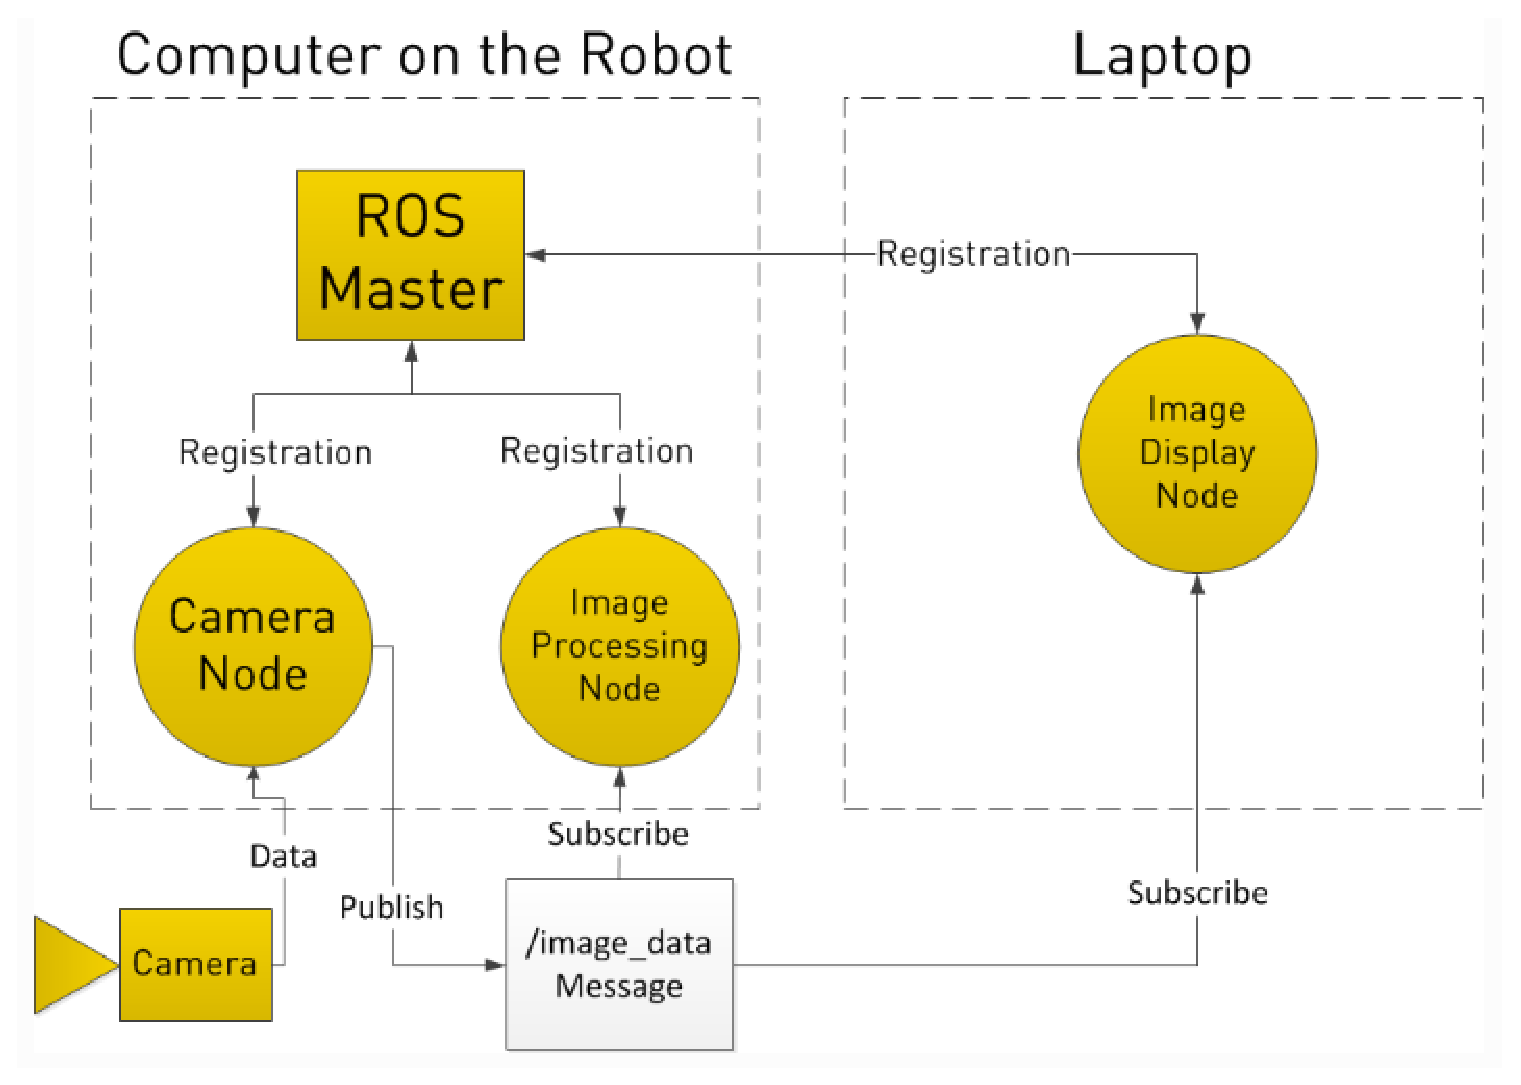
\includegraphics[width=0.8\textwidth]{images/cap3/RosDiagrama.eps}
    \captionof{figure}{Ejemplo de captura de imágenes}
    \label{fig:Ros-Diagram-Example}
\end{minipage}

%+++++++++++++++++++++++++++++++++++++++++++++++++++++++++++++++++++++++++++++++
\subsection{Características}
ROS proporciona un gran número de librerías para resolver los problemas comunes
en el desarrollo robótico con el objetivo de simplificar el la dura carga de
tiempo y trabajo que eso supone \cite{ROSInfraestructura}. Estas son algunas de
las principales características:

\begin{itemize}
  \item \textbf{Mensajes estándar:} existe una gran variedad de mensajes básicos
  ya definidos para la mayoría de tareas del robot como la pose, coordenadas de
  transformación, sensores, odometría, mapas, etc. 
  \item \textbf{Geometría del robot:} la librería \textit{``tf"} se encarga de
  detectar
  las diferentes partes de un robot frente al resto de ellas, siendo posible
  coordinar y transformar más de cien grados de libertad.
  \item \textbf{Lenguaje de descripción:} ROS permite describir las
  particularidades de un robot de una manera redactable. Para ello se usa URDF
  (Unified Robot Description Format), un lenguaje de descripción basado en XML
  que describe todas las características físicas del robot como el tamaño de las
  ruedas, la distancia entre los diferentes componentes e incluso la apariencia
  visual de cada elemento.
  \item \textbf{Diagnóstico:} se ha diseñado un sistema capaz de recoger toda la
  información del robot, para poder registrar, analizar y resolver cualquier
  problema presente en el estado del robot.
  \item \textbf{Navegación:} la mayoría de problemas en la navegación de un
  robot como la estimación de la pose, la localización en un mapa y la
  construcción del misma, son fácilmente resolubles mediante los paquetes que
  proporciona ROS sin necesidad de buscar soluciones propias o de terceros.
\end{itemize}

%+++++++++++++++++++++++++++++++++++++++++++++++++++++++++++++++++++++++++++++++
\subsection{Herramientas}
Una de las características más importantes de ROS está en las herramientas de
desarrollo disponibles. Existe una gran variedad de software de todo tipo:
visualización, depuración, resumen del estado, etc. Gracias al mecanismo de
publicación/suscripción es muy sencillo observar y depurar lo que está
ocurriendo en todo momento.

Por otra parte, ROS puede ser utilizado sin necesidad de usar una interfaz
gráfica (GUI). Toda las características y funcionalidades de ROS pueden
realizarse a través de más de 45 comandos en consola: lanzar grupos de nodos,
examinar tópicos y servicios, grabar y reproducir bolsas de datos, etc. En
cualquier otro caso existe una importante variedad de herramientas con interfaz
gráfica que extienden la funcionalidad de estos comandos. A continuación se
pueden ver algunos de ellos.

%--------------------------------------
\paragraph{RTAB-Map ROS} \hspace{0pt}

Esta herramienta es una extensión del software original RTAB-Map. RTAB-Map
es un aprovechamiento de las técnicas de SLAM capaz de detectar los cierres de
bucles en la navegación de un robot a partir de la apariencia de las imágenes,
los cuales son registrados en un grafo que representa el mapa. Por otra parte,
permite la reconstrucción tridimensional del mapa, el cuál es representado como
una nube de puntos \cite{RTABMap}. 

ROS cuenta con RTABMapviz para visualizar de forma gráfica el resultado de la
detección de los cierres de bucle y la generación en vivo del mapa
tridimensional.

%--------------------------------------
\paragraph{RViz} \hspace{0pt}

RViz es una herramienta de propósito general que permite visualizar en un
espacio tridimensional mucho de los elementos de un robot como ruedas, brazos o
sensores láser. RViz también puede visualizar diferentes mensajes comunes de ROS
como barridos láser, nube de puntos, las imágenes de las cámaras o también con
la posibilidad de mostrar el mapa del entorno (previamente almacenado).

RViz también puede interactuar con la información de la biblioteca
\textit{``tf"} para mostrar toda la información del sistema de coordenadas de
los sensores desde diferentes perspectivas. Entre las ventajas, destaca que se
trata de una herramienta muy importante ya que permite visualizar que ocurre en
el robot en cada momento en busca de errores.

%--------------------------------------
\paragraph{RQt} \hspace{0pt}

RQt es un framework escrito en Qt como el nombre indica que permite desarrollar
aplicaciones personalizadas con interfaz gráfica para cualquier robot. RQt trae
consigo una gran variedad de plugins y/o utilidades para trabajar, de esta forma
cualquier usuario puede modificar según sus necesidades la apariencia y
distribución de estos. Aunque también es posible escribir nuevos plugins
ajustados a la medida de cualquier usuario.

Entre los principales plugins, destacan:

\begin{itemize}
  \item \textbf{rqt\_image\_view:} se trata de la adaptación del paquete de ROS
  'image\_view. Permite visualizar todas las imágenes disponibles en los
  diferentes tópicos activos, tanto imágenes normales, como imágenes en
  estéreo e imágenes de disparidad.
  \item \textbf{rqt\_bag:} permite grabar y gestionar bolsas de datos. Una bolsa
  en formato que permite almacenar todos tipo de datos previamente grabados como
  la lectura de sensores, las imágenes capturadas o el sistema de coordenadas
  utilizado. Son de gran utilidad para depurar y comparar con otras bolsas, ya
  que se pueden visualizar siempre que se deseen sin necesidad de utilizar el
  robot que se utilizó.
  \item \textbf{rqt\_graph:} muestra el estado actual del sistema en forma de
  grafo, como los nodos y las conexiones entre ellos, siendo de gran utilidad
  para la depuración de errores ya que son una forma rápida de ver que todo está
  el sistema está conectado correctamente.
  \item \textbf{rqt\_reconfigure:} adaptación del
  paquete\textit{``dynamic\_reconfigure"} que que permite modificar en tiempo
  real todos los parámetros de los nodos, para realizar modificaciones rápidas
  al vuelo. La configuración de los parámetros se puede exportar para utilizar
  en el futuro.
\end{itemize}

%+++++++++++++++++++++++++++++++++++++++++++++++++++++++++++++++++++++++++++++++

